\section{Disaggregate Hardware Resource}
\label{sec:lego:motivation}

{    
\begin{figure}[h]
\begin{subfigure}{2.5in}
    \begin{center}
    \centerline{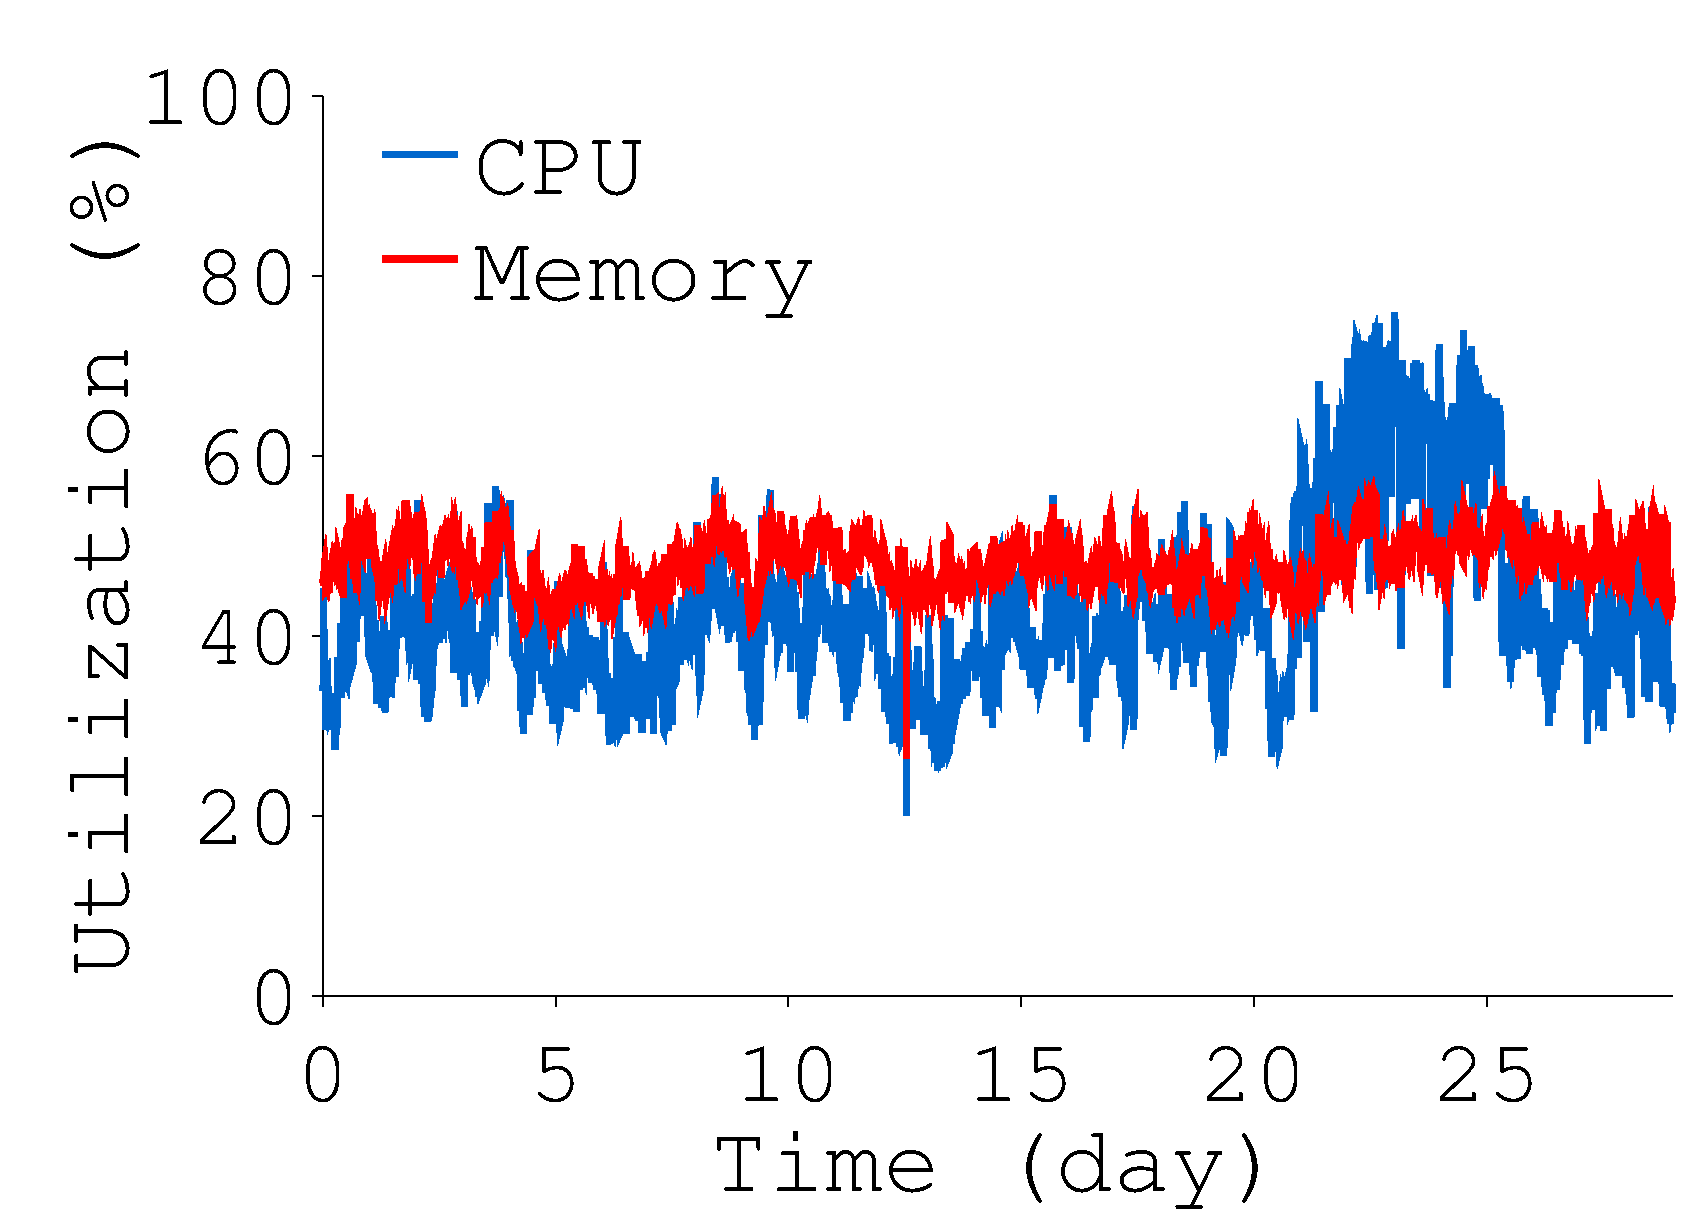
\includegraphics[width=2.5in]{lego/Figures/g_plot_google_util.pdf}}
    \caption[Google Cluster.]{Google Cluster.}
    \label{fig-googleutil}    
    \end{center}
\end{subfigure}
\begin{subfigure}{2.5in}
    \begin{center}    
    \centerline{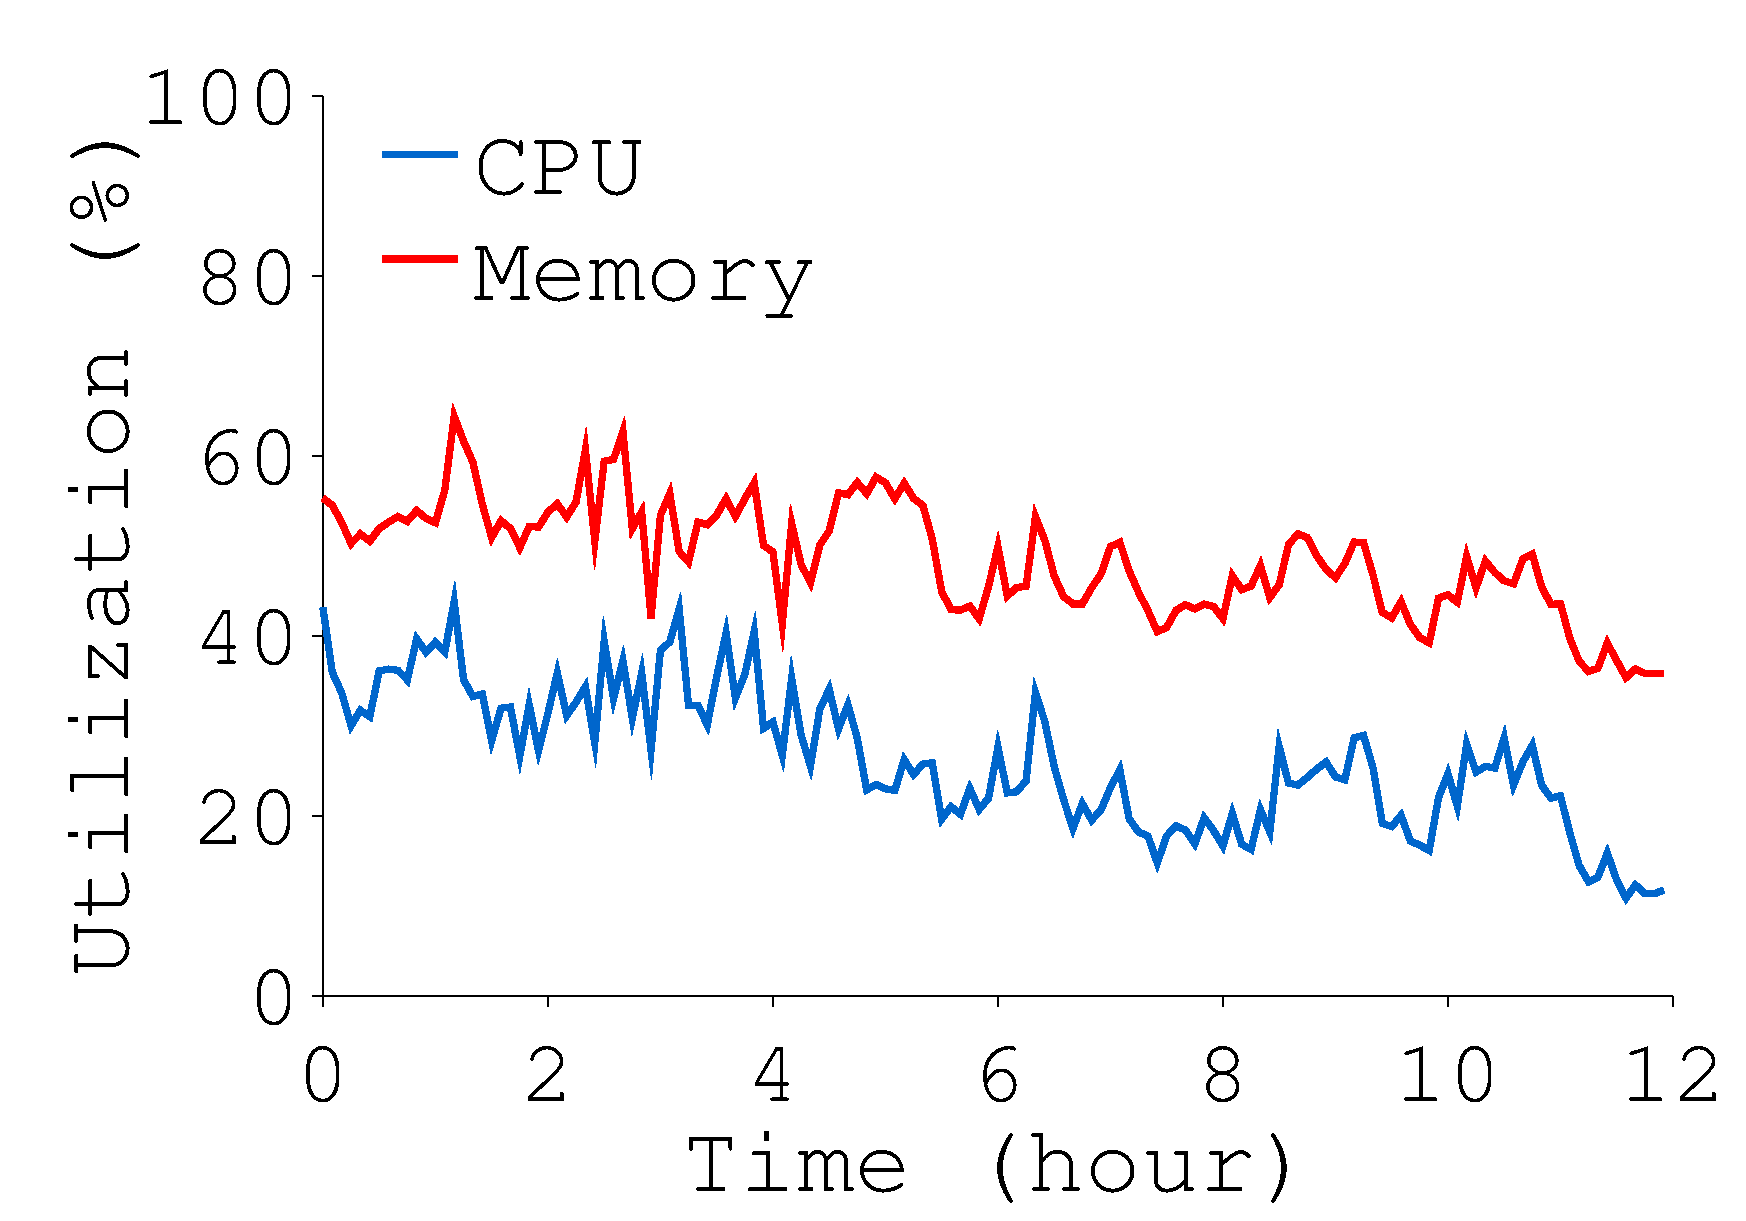
\includegraphics[width=2.5in]{lego/Figures/g_plot_ali_util.pdf}}    
    \caption[Alibaba Cluster.]{Alibaba Cluster.}
    \label{fig-aliutil}
    \end{center}    
\end{subfigure}
\caption[Data center resource utilization.]{Data center resource utilization.}
\label{fig-resource-anal}
\end{figure}
}
{
\begin{figure*}[th]
\begin{subfigure}{1.7in}
\begin{center}
\centerline{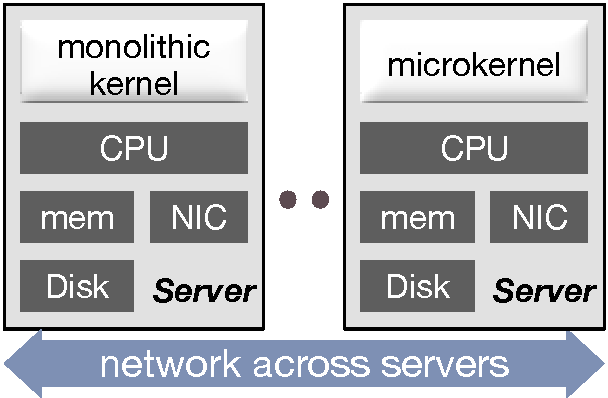
\includegraphics[width=1.7in]{lego/Figures/monolithic-arch.pdf}}
\caption[Monolithic OS.]{OSes Designed for Monolithic Servers.}
\label{fig-monolithic}
\end{center}
\end{subfigure}
\begin{minipage}{0.05in}
\hspace{0.05in}
\end{minipage}
\begin{subfigure}{1.8in}
\begin{center}
\centerline{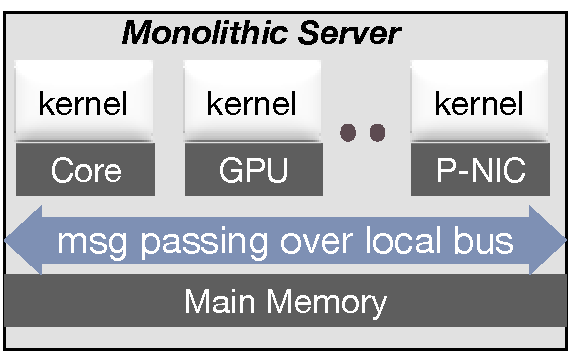
\includegraphics[width=1.8in]{lego/Figures/multikernel-arch.pdf}}
\caption[Multikernel Architecture.]{Multi-kernel Architecture. \small{P-NIC: programmable NIC.}}
\label{fig-multikernel}
\end{center}
\end{subfigure}
\begin{minipage}{0.05in}
\hspace{0.05in}
\end{minipage}
\begin{subfigure}{2.5in}
\begin{center}
\centerline{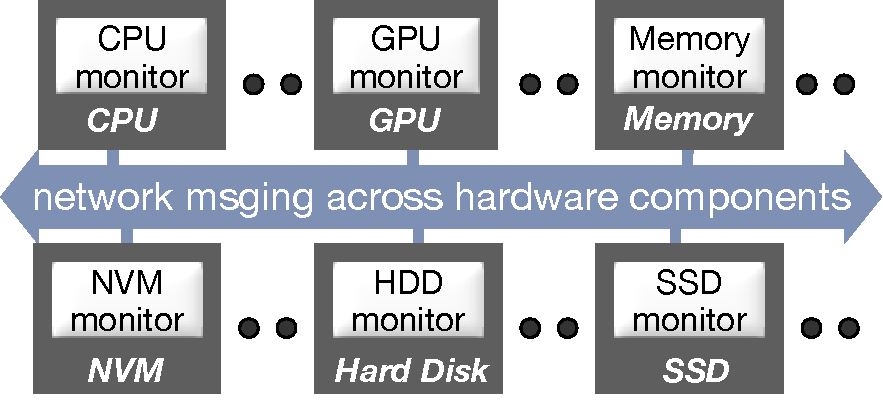
\includegraphics[width=2.6in]{lego/Figures/lego-arch.pdf}}
\caption[Splitkernel Architecture.]{Splitkernel Architecture.}
\label{fig-splitkernel}
\end{center}
\end{subfigure}
\caption[Operating System Architecture.]{Operating System Architecture.}
\end{figure*}
}

This section
motivates the hardware resource disaggregation architecture
and discusses the challenges in managing disaggregated hardware.

\subsection{Limitations of Monolithic Servers}
\label{sec:lego:monolimit}
A monolithic server has been the unit of deployment and operation in datacenters for decades.
This long-standing {\em server-centric} architecture has several key limitations.

\noindent{\textit{\uline{Inefficient resource utilization.}}}
With a server being the physical boundary of resource allocation, 
it is difficult to fully utilize all resources in a datacenter~\cite{Barroso-COMPUTER,Quasar-ASPLOS,PowerNap}.
We analyzed two production cluster traces: a 29-day Google one~\cite{GoogleTrace}
and a 12-hour Alibaba one~\cite{AliTrace}.
Figure~\ref{fig-resource-anal} plots the aggregated CPU and memory utilization in the two clusters.
For both clusters, only around half of the CPU and memory are utilized.
Interestingly,
a significant amount of jobs are being evicted at the same time in these traces
(\eg, evicting low-priority jobs to make room for high-priority ones~\cite{Borg}).
One of the main reasons for resource under-utilization in these production clusters is 
the constraint that CPU and memory for a job have to be allocated from 
the same physical machine.

\noindent{\textit{\uline{Poor hardware elasticity.}}}
It is difficult to add, move, remove, or reconfigure hardware components
after they have been installed in a monolithic server~\cite{FB-Wedge100}. %, and
Because of this rigidity, datacenter owners have to plan out server configurations in advance.
However, with today's speed of change in application requirements, such plans have to be adjusted frequently,
and when changes happen, it often comes with waste in existing server hardware.

\noindent{\textit{\uline{Coarse failure domain.}}}
The failure unit of monolithic servers is coarse.
When a hardware component within a server fails, %(\eg, processor, memory chip, RAID controller), 
the whole server is often unusable and applications running on it can all crash.
Previous analysis~\cite{Failure-Disk-FAST07} found that motherboard, memory, CPU, power supply failures account for 
50\% to 82\% of hardware failures in a server.
Unfortunately, monolithic servers cannot continue to operate when any of these devices fail.

\noindent{\textit{\uline{Bad support for heterogeneity.}}}
Driven by application needs, new hardware technologies are finding their ways into modern datacenters~\cite{sigarch-dc}.
Datacenters no longer host only commodity servers with CPU, DRAM, and hard disks. 
They include non-traditional and specialized hardware like GPGPU~\cite{GPU-google,GPU-aws}, 
TPU~\cite{TPU}, 
DPU~\cite{DPU},
FPGA~\cite{Putnam14-FPGA,Amazon-F1}, %,SmartNIC-nsdi18},
non-volatile memory~\cite{Intel3DXpoint}, %,facebook-eurosys18},
and NVMe-based SSDs~\cite{everspin}.
The monolithic server model tightly couples hardware devices with each other and with a motherboard.
As a result, making new hardware devices work with existing servers is a painful and lengthy process~\cite{Putnam14-FPGA}.
%The current practice of making new hardware work is not only slow but also expensive.
Mover, datacenters often need to purchase new servers to host certain hardware.
Other parts of the new servers can go underutilized 
and old servers need to retire to make room for new ones.

\subsection{Hardware Resource Disaggregation}
The server-centric architecture is a bad fit for the fast-changing datacenter hardware, software, and cost needs.
There is an emerging interest in utilizing resources beyond a local machine~\cite{Gao16-OSDI},
such as distributed memory~\cite{Dragojevic14-FaRM,Nelson15-ATC,Aguilera17-SOCC,Novakovic16-SOCC} and network swapping~\cite{GU17-NSDI}. 
These solutions improve resource utilization over traditional systems.
However, they cannot solve all the issues of monolithic servers (\eg, the last three issues in \S\ref{sec:lego:monolimit}), 
since their hardware model is still a monolithic one.
To fully support the growing heterogeneity in hardware and to provide elasticity and flexibility at the hardware level, 
we should {\em break the monolithic server model.}% into flexible resource components.

We envision a {\em hardware resource disaggregation} architecture 
where hardware resources in traditional servers are disseminated into network-attached {\em hardware components}.
Each component has a controller and a network interface,
can operate on its own,
and is an {\em independent, failure-isolated} entity.

The disaggregated approach largely increases the flexibility of a datacenter.
Applications can freely use resources from any hardware component,
which makes resource allocation easy and efficient.
Different types of hardware resources can {\em scale independently}.
It is easy to add, remove, or reconfigure components.
New types of hardware components can easily be deployed in a datacenter ---
by simply enabling the hardware to talk to the network and adding a new network link to connect it.
Finally, hardware resource disaggregation enables fine-grain failure isolation, % because of decomposed hardware resources.
since one component failure will not affect the rest of a cluster.

Three hardware trends are making resource disaggregation feasible in datacenters.
First, network speed has grown by more than an order of magnitude and has become more scalable in the past decade % faster both in bandwidth and latency
with new technologies like Remote Direct Memory Access ({\it RDMA})~\cite{ibverbs} 
and new topologies and switches~\cite{FireBox-FASTKeynote,costa15-r2c2,Costa-WRSC14},
enabling fast accesses of hardware components that are disaggregated across the network.
InfiniBand will soon reach 200Gbps and sub-600 nanosecond speed~\cite{Mellanox-ConnectX6-IB},
being only 2\x\ to 4\x\ slower than main memory bus in bandwidth.
With main memory bus facing a bandwidth wall~\cite{BW-Wall-ISCA09},
future network bandwidth (at line rate) is even projected to exceed local DRAM bandwidth~\cite{CacheCloud-hotcloud18}.

Second, network interfaces are moving closer to hardware components,
with technologies like Intel OmniPath~\cite{OmniPath},
RDMA~\cite{ibverbs},
and NVMe over Fabrics~\cite{NVMe-fabrics-Inteltalk,NVMe-fabrics}.
As a result, hardware devices will be able to access network directly 
without the need to attach any processors. 

Finally, hardware devices are incorporating more processing power~\cite{Ahn15-PIM,Bojnordi12,Mellanox-SmartNIC,Mellanox-SmartNIC2,Agilio-SmartNIC,Junwhan-ISCA17},
allowing application and OS logics to be offloaded to hardware~\cite{Willow,Kaufmann16-ASPLOS}.
On-device processing power will enable system software to manage disaggregated hardware components locally.

With these hardware trends and the limitations of monolithic servers,
we believe that future datacenters will be able to largely benefit from hardware resource disaggregation.
In fact, there have already been several initial hardware proposals in resource disaggregation~\cite{OCP},
including disaggregated memory~\cite{Lim09-disaggregate,Scaleout-numa,Nitu18-EUROSYS}, 
disaggregated flash~\cite{FlashDisaggregation,ReFlex},
%new power state for disaggregated memory~\cite{Nitu18-EUROSYS},
Intel Rack-Scale System~\cite{IntelRackScale}, 
HP ``The Machine''~\cite{HP-TheMachine,HP-MemoryOS}, 
IBM Composable System~\cite{IBM-Composable},
and Berkeley Firebox~\cite{FireBox-FASTKeynote}.

\subsection{OSes for Resource Disaggregation}
Despite various benefits hardware resource disaggregation promises, 
it is still unclear how to manage or utilize disaggregated hardware in a datacenter.
Unfortunately, existing OSes and distributed systems cannot work well with this new architecture.
Single-node OSes like Linux view a server as the unit of management and assume all hardware components are local (Figure~\ref{fig-monolithic}).
A potential approach is to run these OSes on processors
and access memory, storage, and other hardware resources remotely.
Recent disaggregated systems like soNUMA~\cite{Scaleout-numa} take this approach.
However, this approach incurs high network latency and bandwidth consumption with remote device management,
misses the opportunity of exploiting device-local computation power,
and makes processors the single point of failure.

Multi-kernel solutions~\cite{Baumann-SOSP09,Barrelfish-DC,Helios-SOSP,fos-SOCC,Hive-SOSP} (Figure~\ref{fig-multikernel}) 
view different cores, processors, or programmable devices within a server separately 
by running a kernel on each core/device and using message passing to communicate across kernels.
These kernels still run in a single server and all access some common hardware resources in the server like memory and the network interface.
Moreover, they do not manage distributed resources or handle failures in a disaggregated cluster. 

There have been various distributed OS proposals,
most of which date decades back~\cite{Amoeba-Experience,Sprite,MOSIX}. %,V-System,Accent-SOSP,DEMOS-SOSP,Charlotte}.
Most of these distributed OSes manage a set of monolithic servers
instead of hardware components.

Hardware resource disaggregation is fundamentally different from the traditional monolithic server model.
A complete disaggregation of processor, memory, and storage 
means that when managing one of them, there will be no local accesses to the other two.
For example, processors will have no local memory or storage to store user or kernel data.
%Memory and storage components will only have limited processing power. %not have no local memory to serve as cache.
An OS also needs to manage distributed hardware resource and handle hardware component failure.
We summarize the following key challenges in building an OS for resource disaggregation,
some of which have previously been identified~\cite{HP-MemoryOS}.

\begin{itemize}
\item How to deliver good performance when application execution involves the access of network-partitioned disaggregated hardware
and current network is still slower than local buses?

\item How to locally manage individual hardware components with limited hardware resources?

%\item How to communicate across components?

\item How to manage distributed hardware resources?

\item How to handle a component failure without affecting other components or running applications?

\item What abstraction should be exposed to users and how to support existing datacenter applications?

\end{itemize}

Instead of retrofitting existing OSes to confront these challenges,
we take the approach of designing a new OS architecture from the ground up for hardware resource disaggregation.
